\documentclass{article}
\usepackage{amsmath}
\usepackage{graphicx}
\usepackage{enumitem}
\usepackage{hyperref}
\usepackage[margin=1in]{geometry}
\usepackage{xcolor}

\title{XAI Techniques Cheatsheet}
\author{Yvo Keller}
\date{\today}

\begin{document}
\maketitle

\pagebreak
\section{Tabular Methods}

\subsection{Method Selection Guide}
\begin{table}[h]
\caption{Comparison of Tabular XAI Methods}
\begin{center}
\resizebox{\textwidth}{!}{
\begin{tabular}{|p{3cm}|p{3cm}|p{3cm}|p{3cm}|}
\hline
\textbf{Use Case} & \textbf{PDP} & \textbf{ICE} & \textbf{Shapley} \\
\hline
Global Feature Effect & Best Choice & Limited & Good \\
\hline
Individual Predictions & Not Suitable & Good & Best Choice \\
\hline
Feature Interactions & Limited & Good & Limited \\
\hline
Categorical Features & Good & Good & Best Choice \\
\hline
Computational Cost & Low & Medium & High \\
\hline
Model Agnostic & Yes & Yes & Yes \\
\hline
\end{tabular}
}
\end{center}
\end{table}

\subsection{Partial Dependence Plots (PDP)}

\subsubsection{Overview}
PDPs show how a feature affects predictions on average, while marginalizing over all other features.

\begin{figure}[h]
    \centering
    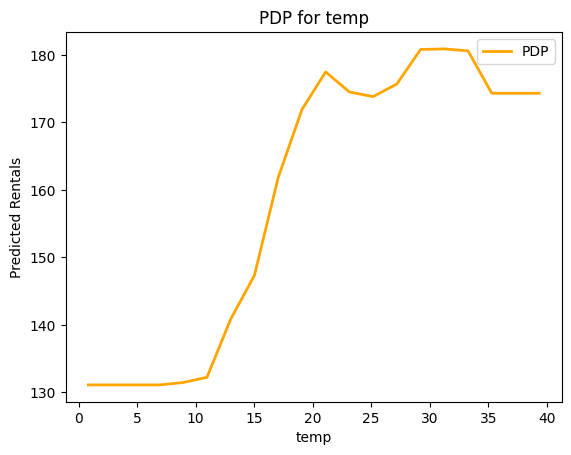
\includegraphics[width=0.8\textwidth]{images/pdp.png}
    \caption{Example of a Partial Dependence Plot (PDP)}
    \label{fig:pdp}
\end{figure}

\subsubsection{Intuitive Example}
Consider our ice cream sales model:
\begin{itemize}
    \item To create a PDP for temperature:
    \begin{enumerate}
        \item Pick a temperature value (e.g., 25°C)
        \item For every data point, set temperature to 25°C
        \item Get model predictions for all these modified points
        \item Average these predictions
        \item Repeat for different temperature values
        \item Plot temperature vs. average predictions
    \end{enumerate}
\end{itemize}

\subsubsection{Interpretation}
\begin{itemize}
    \item Slope shows relationship strength
    \item Shape reveals non-linear effects
    \item Flat regions indicate no impact
    \item Limitations: Can miss feature interactions
\end{itemize}

\subsection{Individual Conditional Expectation (ICE) Plots / ICPs}

\subsubsection{Overview}
ICE plots (also known as ICPs) extend PDPs by showing how predictions change for individual instances, revealing heterogeneous effects hidden by PDPs.

\begin{figure}[h]
    \centering
    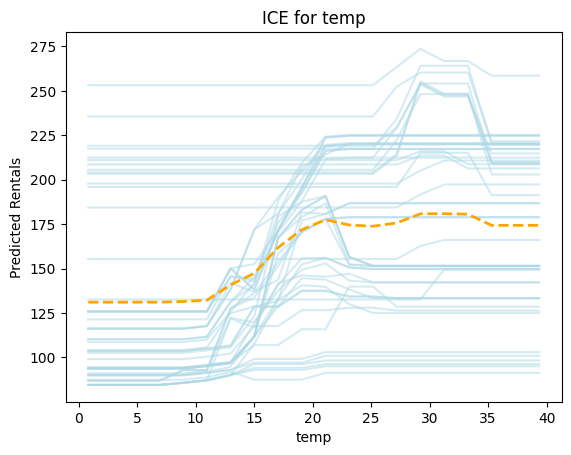
\includegraphics[width=0.8\textwidth]{images/ice.png}
    \caption{Example of Individual Conditional Expectation (ICE) plots}
    \label{fig:ice}
\end{figure}

\subsubsection{Intuitive Example}
Using our ice cream model:
\begin{itemize}
    \item For each individual day in our dataset:
    \begin{enumerate}
        \item Keep all features fixed except temperature
        \item Vary temperature across its range
        \item Plot prediction line for this specific day
    \end{enumerate}
    \item Result: Multiple lines, one per instance
    \item PDP would be the average of these lines
\end{itemize}

\subsubsection{Key Insights}
\begin{itemize}
    \item Diverging lines suggest feature interactions
    \item Parallel lines indicate consistent effects
    \item Crossing lines show complex relationships
    \item More informative than PDP alone
\end{itemize}

\subsubsection{When to Use}
\begin{itemize}
    \item Feature interaction analysis
    \item Detecting heterogeneous effects
    \item Model behavior validation
    \item Identifying outlier instances
\end{itemize}

\subsection{Shapley Values}

\subsubsection{Overview}
Shapley values provide a way to fairly distribute the prediction among features by considering all possible feature combinations.

\subsubsection{Key Formula}
The Shapley value for feature $i$ is:
\begin{equation}
    \phi_i(x) = \sum_{S \subseteq N \backslash\{i\}} \frac{|S|!\times(|N|-|S|-1)!}{|N|!}\left(f_\theta(S \cup\{i\})-f_\theta(S)\right)
\end{equation}

where:
\begin{itemize}
    \item $N$ is the set of all features
    \item $S$ is a subset of features excluding feature $i$
    \item $f_\theta$ is the model prediction
    \item $|S|$ is the size of subset $S$
    \item $|N|$ is the total number of features
\end{itemize}

\subsubsection{Calculation Process}
\begin{enumerate}
    \item Select an instance to explain
    \item For each feature:
    \begin{enumerate}
        \item Generate all possible feature coalitions excluding the target feature
        \item For each coalition:
        \begin{enumerate}
            \item Calculate model prediction with and without target feature
            \item Compute marginal contribution
            \item Weight contribution by coalition size
        \end{enumerate}
        \item Sum weighted contributions
    \end{enumerate}
    \item Average contributions over all permutations
\end{enumerate}

\subsubsection{Properties}
\begin{itemize}
    \item \textbf{Efficiency}: Sum of Shapley values equals model output minus baseline
    \item \textbf{Symmetry}: Equal contribution features receive equal Shapley values
    \item \textbf{Dummy}: Features with no marginal contribution get zero Shapley value
    \item \textbf{Additivity}: Values can be computed independently and summed
\end{itemize}

\subsubsection{Intuitive Example: Ice Cream Shop}
Let's understand Shapley values through a practical example of predicting ice cream sales.

\paragraph{Setup}
Consider a model predicting daily ice cream sales with features:
\begin{itemize}
    \item $x_1$ = Day of the week
    \item $x_2$ = Number of flights arriving
    \item $x_3$ = Temperature
    \item $x_4$ = Total opening hours
\end{itemize}

\paragraph{Calculation Process}
To calculate the Shapley value for temperature ($x_3$):

\begin{enumerate}
    \item \textbf{Select a sample}: Choose a specific day's data point
    \item \textbf{Choose baseline}: Select a reference point (usually average values)
    \item \textbf{Generate permutation}: e.g., $(x_4, x_1, x_3, x_2)$
    \item \textbf{Calculate marginal contributions}:
    \begin{itemize}
        \item Start with baseline prediction: $f_\text{base}$
        \item Add features one by one:
            \begin{align*}
                &f(x_4) \\
                &f(x_4, x_1) \\
                &f(x_4, x_1, x_3) \leftarrow \text{Temperature added here} \\
                &f(x_4, x_1, x_3, x_2)
            \end{align*}
        \item Temperature's contribution = $f(x_4, x_1, x_3) - f(x_4, x_1)$
    \end{itemize}
    \item \textbf{Repeat}: Do this for multiple permutations
    \item \textbf{Average}: The Shapley value is the average contribution across permutations
\end{enumerate}

\paragraph{Interpretation}
The final Shapley value for temperature tells us:
\begin{itemize}
    \item Positive value: Higher temperatures increase ice cream sales
    \item Negative value: Higher temperatures decrease sales
    \item Magnitude: Size of temperature's impact on the prediction
\end{itemize}

\subsubsection{Monte Carlo Approximation}
For large feature sets, exact computation becomes infeasible. Monte Carlo approximation:
\begin{enumerate}
    \item Sample random feature permutations
    \item Calculate marginal contributions for each permutation
    \item Average results over all samples
\end{enumerate}

\subsubsection{SHAP Summary Plot (Beeswarm)}
\begin{figure}[h]
    \centering
    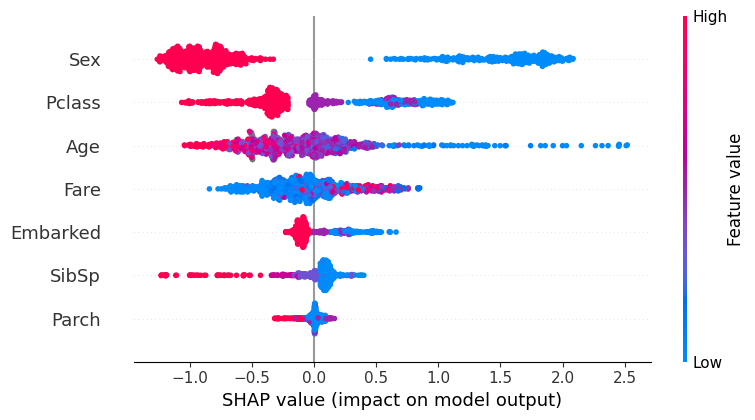
\includegraphics[width=0.8\textwidth]{images/bee_swarm.png}
    \caption{SHAP Summary Plot showing feature importance and impact distribution}
    \label{fig:shap_summary}
\end{figure}

\paragraph{How to Read the Plot}
\begin{itemize}
    \item \textbf{Target}: The model predicts passenger survival probability (0 = died, 1 = survived)
    \item \textbf{Feature Ranking}: Features are ordered by their absolute impact on survival prediction (most important at top)
    \item \textbf{Impact}: The x-axis shows SHAP values (impact on survival probability)
        \begin{itemize}
            \item Positive values (right) increase survival probability
            \item Negative values (left) decrease survival probability
            \item The magnitude shows how strongly it affects the prediction
        \end{itemize}
    \item \textbf{Distribution}: Each dot is one passenger in the dataset
    \item \textbf{Color Coding}:
        \begin{itemize}
            \item For categorical features (like Sex): Blue/Red represent different categories
            \item For numerical features: Red = high values, Blue = low values
            \item Look at the pattern of colors and their position to understand the relationship
        \end{itemize}
    \item \textbf{Spread}: Horizontal spread shows range of impact across different passengers
\end{itemize}

\paragraph{Example Interpretation}
Looking at the Titanic survival predictions:
\begin{itemize}
    \item \textbf{Sex}: Strongest predictor of survival
        \begin{itemize}
            \item Being female (blue) strongly increased survival probability (dots on right)
            \item Being male (red) strongly decreased survival probability (dots on left)
            \item Clear separation shows this was the most decisive factor
        \end{itemize}
    \item \textbf{Pclass}: Second most important feature
        \begin{itemize}
            \item First class (blue = low class number) increased survival probability
            \item Third class (red = high class number) decreased survival probability
            \item Shows clear socioeconomic divide in survival chances
        \end{itemize}
    \item \textbf{Age}: Complex relationship
        \begin{itemize}
            \item Younger passengers (blue) show mixed effects but often positive
            \item Older passengers (red) tend toward negative impact on survival
            \item Wide spread suggests age interacted with other factors
        \end{itemize}
    \item \textbf{Fare}: Shows price paid for ticket
        \begin{itemize}
            \item Higher fares (red) tend toward positive impact
            \item Lower fares (blue) tend toward negative impact
            \item Considerable overlap in the middle ranges
        \end{itemize}
    \item \textbf{Embarked}: Port where passenger boarded
        \begin{itemize}
            \item Different ports (shown by different colors) had varying impacts
            \item Moderate but clear influence on survival chances
        \end{itemize}
    \item \textbf{SibSp \& Parch}: Number of family members aboard
        \begin{itemize}
            \item More family members (red) shows mixed effects
            \item Fewer family members (blue) also shows varied impact
            \item Wide spread suggests complex relationship with survival
        \end{itemize}
\end{itemize}

\pagebreak
\section{Text Data Methods}

\subsection{Method Selection Guide}
\begin{table}[h]
\caption{Comparison of Text XAI Methods}
\begin{center}
\small
\begin{tabular}{|l|c|c|c|c|}
\hline
\textbf{Use Case} & \textbf{LIME} & \textbf{Gradient × Input} & \textbf{Attention} & \textbf{Embeddings} \\
\hline
Local Explanations & Best Choice & Good & Limited & Not Suitable \\
\hline
Token Importance & Good & Best Choice & Good & Not Suitable \\
\hline
Word Relationships & Not Suitable & Limited & Best Choice & Good \\
\hline
Model Understanding & Limited & Limited & Good & Best Choice \\
\hline
Computation Speed & Slow & Fast & Fast & Medium \\
\hline
Model Agnostic & Yes & No & No & Partial \\
\hline
\end{tabular}
\end{center}
\end{table}

\subsection{LIME (Local Interpretable Model-agnostic Explanations)}

\subsubsection{Overview}
LIME explains individual text predictions by approximating the complex model locally with an interpretable one.

\subsubsection{How it Works}
\begin{enumerate}
    \item \textbf{Input}: Take a text instance to explain
    \item \textbf{Perturbation}: 
        \begin{itemize}
            \item Create variations of the input by removing words
            \item Keep track of which words are present/absent
        \end{itemize}
    \item \textbf{Prediction}: Get model predictions for all variations
    \item \textbf{Local Model}: 
        \begin{itemize}
            \item Fit an interpretable model (e.g., linear) around the instance
            \item Weight samples by proximity to original text
        \end{itemize}
    \item \textbf{Explanation}: Show which words contributed positively/negatively
\end{enumerate}

\subsubsection{Example Interpretation}
For a sentiment analysis model:
\begin{itemize}
    \item Positive words might be highlighted in green
    \item Negative words might be highlighted in red
    \item Weight of highlighting shows importance
    \item Example: ``The movie was {\color{green}great} but the ending was {\color{red}disappointing}''
\end{itemize}

\subsection{Gradient × Input}

\subsubsection{Overview}
Gradient × Input identifies important words by computing how much a small change in each input token would affect the prediction.

\subsubsection{Calculation}
\begin{enumerate}
    \item Calculate gradient of output with respect to input embeddings
    \item Multiply gradient by the actual input embeddings
    \item Aggregate for each token (usually L2 norm across embedding dimensions)
\end{enumerate}

\subsubsection{Properties}
\begin{itemize}
    \item \textbf{Advantages}:
        \begin{itemize}
            \item Computationally efficient
            \item Exact gradient computation
            \item Works with any differentiable model
        \end{itemize}
    \item \textbf{Limitations}:
        \begin{itemize}
            \item Can be noisy
            \item May not capture non-linear interactions well
            \item Requires model gradients
        \end{itemize}
\end{itemize}

\subsection{Attention Matrices}

\subsubsection{Overview}
Attention matrices visualize how different parts of the input text relate to each other in transformer-based models.

\begin{figure}[h]
    \centering
    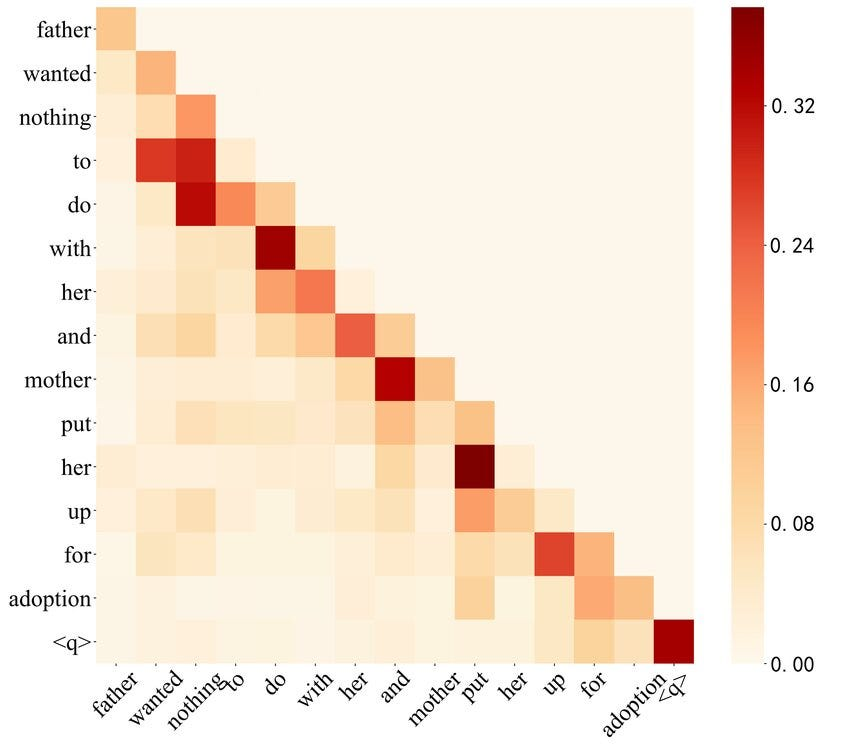
\includegraphics[width=0.8\textwidth]{images/am.jpg}
    \caption{Example of an Attention Matrix showing token relationships in a transformer model}
    \label{fig:attention_matrix}
\end{figure}

\subsubsection{Components}
\begin{itemize}
    \item \textbf{Attention Heads}:
        \begin{itemize}
            \item Each head learns different relationship patterns
            \item Multiple heads capture different aspects of the text
        \end{itemize}
    \item \textbf{Attention Weights}:
        \begin{itemize}
            \item Show how much each token attends to other tokens
            \item Higher weights indicate stronger relationships
        \end{itemize}
    \item \textbf{Layers}:
        \begin{itemize}
            \item Earlier layers often capture syntactic relationships
            \item Later layers tend to capture semantic relationships
        \end{itemize}
\end{itemize}

\subsubsection{Visualization}
\begin{itemize}
    \item Usually shown as a heatmap matrix
    \item Rows: Source tokens
    \item Columns: Target tokens
    \item Color intensity: Attention weight
    \item Can be aggregated across heads or shown per head
\end{itemize}

\subsubsection{Example Patterns}
\begin{itemize}
    \item \textbf{Diagonal}: Token attending to itself
    \item \textbf{Vertical stripes}: Important context words
    \item \textbf{Horizontal stripes}: Influential tokens
    \item \textbf{Blocks}: Related phrase chunks
    \item \textbf{Off-diagonal}: Long-range dependencies
\end{itemize}

\subsubsection{Interpretation Tips}
\begin{itemize}
    \item Look for consistent patterns across multiple heads
    \item Compare patterns at different layers
    \item Consider linguistic relationships (e.g., subject-verb, coreference)
    \item Be cautious: attention $\neq$ causation
    \item Use in conjunction with other explanation methods
\end{itemize}

\subsection{Embedding Visualization (T-SNE and PCA)}

\subsubsection{Overview}
These techniques help visualize high-dimensional word/token embeddings in 2D/3D space, making it possible to understand relationships between words and how the model represents language.

\subsubsection{Key Methods}
\begin{itemize}
    \item \textbf{PCA (Principal Component Analysis)}:
        \begin{itemize}
            \item Linear dimensionality reduction
            \item Preserves global structure and distances
            \item Faster but may miss non-linear relationships
        \end{itemize}
    \item \textbf{T-SNE (t-Distributed Stochastic Neighbor Embedding)}:
        \begin{itemize}
            \item Non-linear dimensionality reduction
            \item Better at preserving local clusters
            \item Shows semantic relationships more clearly
        \end{itemize}
\end{itemize}

\subsubsection{Interactive Tool}
The TensorFlow Embedding Projector (\url{projector.tensorflow.org}) allows:
\begin{itemize}
    \item Interactive exploration of embeddings
    \item Switching between PCA and T-SNE views
    \item Finding nearest neighbors
    \item Visualizing word clusters and relationships
\end{itemize}

\subsection{Language Interpretability Tool (LIT)}

\subsubsection{Overview}
LIT is an interactive platform for analyzing NLP models, combining multiple interpretation techniques in one interface.

\subsubsection{Key Features}
\begin{itemize}
    \item \textbf{Model Analysis}:
        \begin{itemize}
            \item Attention visualization
            \item Salience maps
            \item Counterfactual generation
        \end{itemize}
    \item \textbf{Dataset Exploration}:
        \begin{itemize}
            \item Data point inspection
            \item Slice analysis
            \item Error analysis
        \end{itemize}
    \item \textbf{Interactive Testing}:
        \begin{itemize}
            \item Real-time predictions
            \item Custom input testing
            \item Model comparison
        \end{itemize}
\end{itemize}

\subsubsection{Use Cases}
\begin{itemize}
    \item Debug model predictions
    \item Identify dataset biases
    \item Compare model versions
    \item Explore model behavior systematically
\end{itemize}

\pagebreak
\section{Image Data Methods}

\subsection{Method Selection Guide}
\begin{table}[h]
\caption{Comparison of Image XAI Methods}
\begin{center}
\resizebox{\textwidth}{!}{
\begin{tabular}{|p{2.5cm}|p{2.5cm}|p{2.5cm}|p{2.5cm}|}
\hline
\textbf{Use Case} & \textbf{Grad-CAM} & \textbf{Integrated Gradients} & \textbf{Occlusion} \\
\hline
Localization & Best Choice & Good & Good \\
\hline
Pixel Attribution & Limited & Best Choice & Good \\
\hline
Model Agnostic & No & No & Yes \\
\hline
Computation Speed & Fast & Medium & Slow \\
\hline
Implementation & Medium & Complex & Simple \\
\hline
Resolution & Limited by Features & Full & Patch-based \\
\hline
\end{tabular}
}
\end{center}
\end{table}

\subsection{Grad-CAM (Gradient-weighted Class Activation Mapping)}

\subsubsection{Core Concept}
Grad-CAM answers the question: "Which regions of an image did the CNN focus on to make its prediction?" It does this by:
\begin{itemize}
    \item Looking at the last convolutional layer's feature maps
    \item Weighting them based on their importance for the target class
    \item Creating a heatmap showing which image regions were most influential
\end{itemize}

\begin{figure}[h]
    \centering
    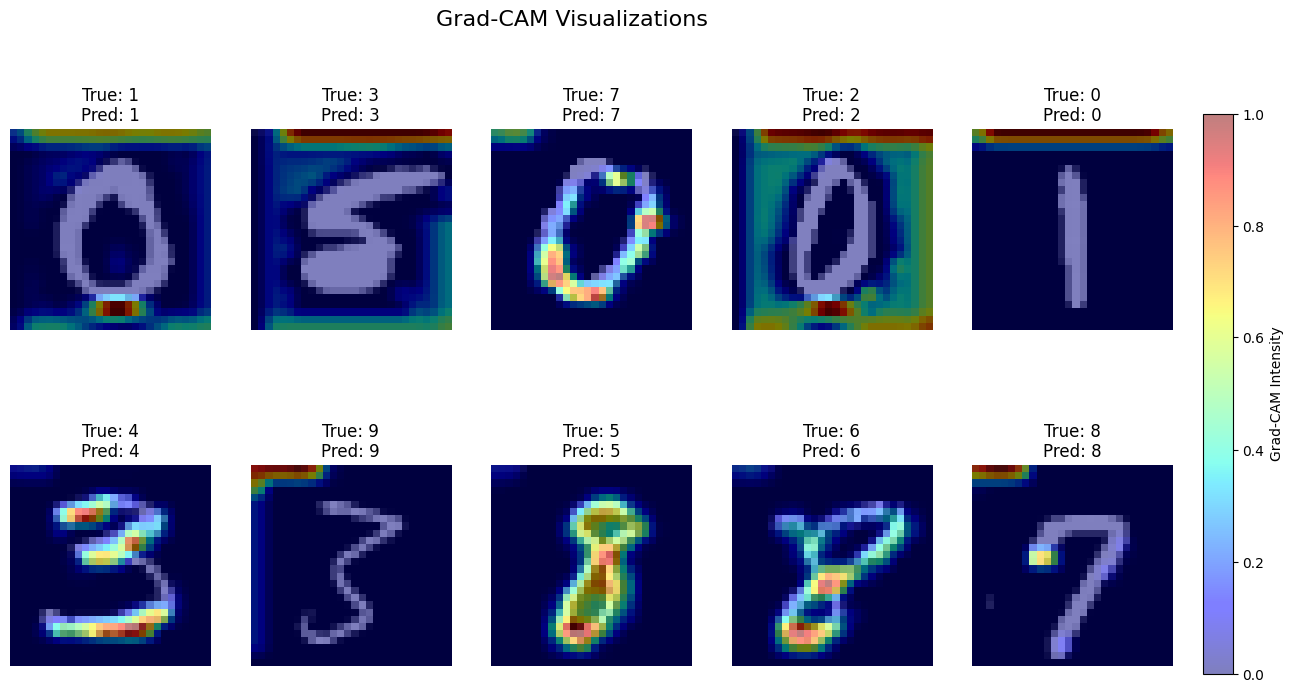
\includegraphics[width=0.8\textwidth]{images/grad_cam.png}
    \caption{Example of Grad-CAM visualization showing regions of interest for classification}
    \label{fig:grad_cam}
\end{figure}

\subsubsection{Why It Works}
\begin{itemize}
    \item Later conv layers capture high-level features
    \item Each feature map specializes in detecting different patterns
    \item Gradients tell us which patterns were important for the specific prediction
    \item Combining this information creates an interpretable visualization
\end{itemize}

\subsubsection{The Process}
\begin{enumerate}
    \item Get feature maps from last conv layer for an input image
    \item Calculate how important each feature map was for the prediction
    \item Create weighted combination of feature maps
    \item Upscale to original image size and overlay
\end{enumerate}

\subsubsection{Technical Implementation}
Based on implementation in \texttt{notebooks/mini\_challenge.ipynb}:

\begin{enumerate}
    \item \textbf{Feature Extraction}:
        \begin{itemize}
            \item Forward pass through CNN
            \item Capture activations at chosen conv layer
        \end{itemize}
    
    \item \textbf{Importance Weights}:
        \begin{itemize}
            \item Compute gradients for target class
            \item Average gradients for each feature map:
            \begin{equation}
                \alpha_k = \frac{1}{Z} \sum_i \sum_j \frac{\partial y^c}{\partial A^k_{ij}}
            \end{equation}
        \end{itemize}
    
    \item \textbf{Create Heatmap}:
        \begin{itemize}
            \item Weight each feature map by its importance
            \item Sum all weighted maps
            \item Apply ReLU to highlight positive contributions:
            \begin{equation}
                L^c_\text{Grad-CAM} = \text{ReLU}\left(\sum_k \alpha_k A^k\right)
            \end{equation}
        \end{itemize}
\end{enumerate}

\subsubsection{Reading the Output}
\begin{itemize}
    \item \textbf{Heatmap Colors}:
        \begin{itemize}
            \item Red regions: Strongly support the prediction
            \item Blue regions: Less important for the prediction
        \end{itemize}
    \item \textbf{What to Look For}:
        \begin{itemize}
            \item Does it focus on meaningful parts?
            \item How focused/dispersed is the attention?
            \item Does it match human intuition?
        \end{itemize}
\end{itemize}

\subsubsection{Key Strengths}
\begin{itemize}
    \item Simple yet effective visualization
    \item Works with any CNN architecture
    \item No need to modify or retrain the model
    \item Class-specific explanations
\end{itemize}

\subsection{Integrated Gradients (IG)}

\subsubsection{Core Concept}
Integrated Gradients answers: "How much did each input feature contribute to the prediction, compared to a baseline?" It does this by:
\begin{itemize}
    \item Considering a path from a baseline (usually zeros) to the actual input
    \item Accumulating gradients along this path
    \item Showing which input features were most influential for the prediction
\end{itemize}

\begin{figure}[h]
    \centering
    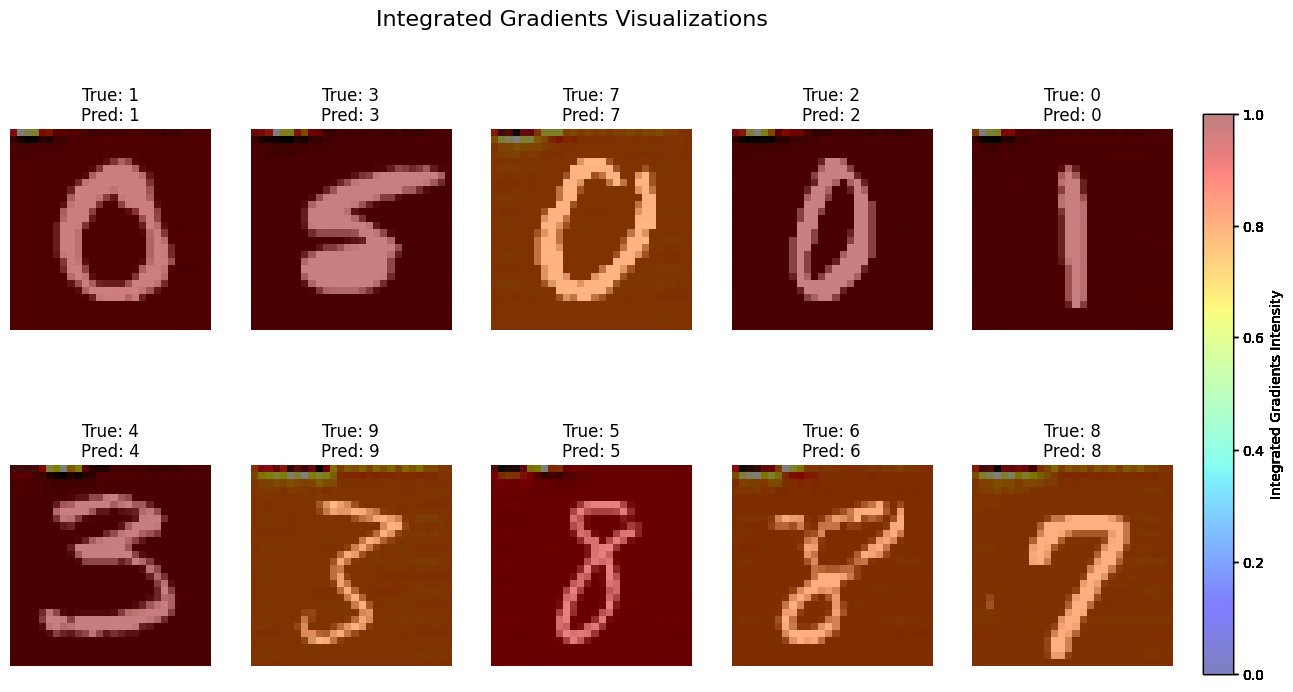
\includegraphics[width=0.8\textwidth]{images/integrated_gradients.png}
    \caption{Example of Integrated Gradients showing pixel-wise contributions to the prediction}
    \label{fig:integrated_gradients}
\end{figure}

\subsubsection{Why It Works}
\begin{itemize}
    \item Gradients at a single point might be noisy or saturated
    \item By integrating over a path, we capture the cumulative effect
    \item The baseline (e.g., black image) serves as a natural reference point
    \item Satisfies important theoretical properties (completeness, symmetry)
\end{itemize}

\subsubsection{The Process}
\begin{enumerate}
    \item Define baseline (e.g., black image)
    \item Create steps between baseline and input
    \item Compute gradients at each step
    \item Average the gradients
    \item Multiply by (input - baseline)
\end{enumerate}

\subsubsection{Mathematical Foundation}
The integrated gradients along the $i$th dimension is:
\begin{equation}
    IG_i(x) = (x_i - x'_i) \times \int_{\alpha=0}^{1} \frac{\partial F(x' + \alpha(x-x'))}{\partial x_i} d\alpha
\end{equation}
where:
\begin{itemize}
    \item $x$ is the input
    \item $x'$ is the baseline
    \item $F$ is the model
    \item $\alpha$ is the interpolation parameter
\end{itemize}

\subsubsection{Technical Implementation}
Based on implementation in \texttt{notebooks/mini\_challenge.ipynb}:

\begin{enumerate}
    \item \textbf{Setup}:
        \begin{itemize}
            \item Define baseline (e.g., zero tensor)
            \item Choose number of steps (e.g., 50)
            \item Identify target class (predicted or specified)
        \end{itemize}
    
    \item \textbf{Path Interpolation}:
        \begin{itemize}
            \item Create scaled inputs between baseline and input:
            \begin{equation}
                x_\alpha = x' + \alpha(x - x') \quad \text{for } \alpha \in [0,1]
            \end{equation}
            \item Discretize path into steps
        \end{itemize}
    
    \item \textbf{Gradient Accumulation}:
        \begin{itemize}
            \item For each step along path:
                \begin{itemize}
                    \item Forward pass through model
                    \item Compute gradients w.r.t. input
                    \item Store gradients
                \end{itemize}
            \item Average all collected gradients
        \end{itemize}
    
    \item \textbf{Final Attribution}:
        \begin{itemize}
            \item Multiply average gradients by (input - baseline)
            \item Result shows per-feature contributions
        \end{itemize}
\end{enumerate}

\subsubsection{Reading the Output}
\begin{itemize}
    \item \textbf{Values}:
        \begin{itemize}
            \item Positive: Feature pushed prediction toward target class
            \item Negative: Feature pushed prediction away from target class
            \item Magnitude: Strength of contribution
        \end{itemize}
    \item \textbf{What to Look For}:
        \begin{itemize}
            \item Which features had strongest contributions
            \item Whether contributions match domain knowledge
            \item Balance between positive and negative contributions
        \end{itemize}
\end{itemize}

\subsubsection{Key Strengths}
\begin{itemize}
    \item Theoretically sound with axiomatic justification
    \item Works for any differentiable model
    \item Provides pixel-level attributions for images
    \item Computationally tractable
\end{itemize}

\subsection{Occlusion Sensitivity Analysis}

\subsubsection{Core Concept}
Occlusion analysis answers: "How does hiding different parts of the image affect the model's prediction?" It does this by:
\begin{itemize}
    \item Systematically blocking out parts of the image
    \item Measuring the change in prediction confidence
    \item Creating a heatmap of importance regions
\end{itemize}

\subsubsection{Why It Works}
\begin{itemize}
    \item Simple and intuitive approach
    \item If hiding a region significantly drops the prediction score, that region was important
    \item Model-agnostic: works with any image classifier
    \item Provides direct evidence of feature importance
\end{itemize}

\subsubsection{The Process}
\begin{enumerate}
    \item Choose occlusion parameters:
        \begin{itemize}
            \item Patch size (e.g., 8x8 pixels)
            \item Stride (how much to move the patch)
            \item Fill value (e.g., gray, black, or blur)
        \end{itemize}
    \item For each position:
        \begin{itemize}
            \item Create copy of image
            \item Replace patch with chosen fill value
            \item Get model's prediction
            \item Record change in confidence
        \end{itemize}
    \item Create heatmap from recorded changes
\end{enumerate}

\subsubsection{Reading the Output}
\begin{itemize}
    \item \textbf{Heatmap Interpretation}:
        \begin{itemize}
            \item Darker regions: Occluding these areas greatly affected prediction
            \item Lighter regions: Less important for the prediction
            \item Size of important regions relates to patch size used
        \end{itemize}
    \item \textbf{What to Look For}:
        \begin{itemize}
            \item Are important regions semantically meaningful?
            \item How do different patch sizes affect the result?
            \item Are there unexpected important regions?
        \end{itemize}
\end{itemize}

\subsubsection{Key Strengths}
\begin{itemize}
    \item Highly intuitive explanation method
    \item No need for model gradients
    \item Can use different occlusion strategies
    \item Easy to implement and debug
\end{itemize}

\subsubsection{Limitations}
\begin{itemize}
    \item Computationally expensive (needs many forward passes)
    \item Results depend on occlusion parameters
    \item May miss fine-grained feature interactions
    \item Rectangular patches might not match object shapes
\end{itemize}

\end{document} 